\documentclass[12pt, a4paper, lithuanian]{article}

\usepackage[utf8x]{inputenc}
\def\LTfontencoding{L7x}
\usepackage[\LTfontencoding]{fontenc}
\usepackage[lithuanian]{babel}

\usepackage{VUMIF}
\usepackage{listings}

% "define" Scala
\lstdefinelanguage{scala}{
  morekeywords={abstract,case,catch,class,def,%
    do,else,extends,false,final,finally,%
    for,if,implicit,import,match,mixin,%
    new,null,object,override,package,%
    private,protected,requires,return,sealed,%
    super,this,throw,trait,true,try,%
    type,val,var,while,with,yield},
  otherkeywords={=>,<-,<\%,<:,>:,\#,@},
  sensitive=true,
  morecomment=[l]{//},
  morecomment=[n]{/*}{*/},
  morestring=[b]",
  morestring=[b]',
  morestring=[b]""
}

\usepackage{color}
\definecolor{dkgreen}{rgb}{0,0.6,0}
\definecolor{gray}{rgb}{0.5,0.5,0.5}
\definecolor{mauve}{rgb}{0.58,0,0.82}


% Default settings for code listings
\lstset{frame=tb,
  language=scala,
  aboveskip=3mm,
  belowskip=3mm,
  showstringspaces=false,
  columns=flexible,
  basicstyle={\small\ttfamily},
  numbers=none,
  numberstyle=\tiny\color{gray},
  %keywordstyle=\color{blue},
  %commentstyle=\color{dkgreen},
  %stringstyle=\color{mauve},
  frame=single,
  breaklines=true,
  breakatwhitespace=true
  tabsize=3
}

% \usepackage[mathcsdepttitle]{VUMIF} % --- matematinės informatikos katedros
%     titulinio puslapio formatavimas

% Titulinio puslapio reikalai
\vumifdept{Informatikos katedra}
\vumifpaper{Mokslo tiriamasis darbas}
\title{Funkcinio-reaktyvaus programavimo taikymas įvykių kaupimo sistemose}
\engtitle{Functional Reactive Programming in Event Sourcing Systems}
\author{
    1 kurso 7 grupės studentas \\
    Žilvinas Kučinskas
}

\supervisor{Viačeslav Pozdniakov}
\reviewer{prof. Rimantas Vaicekauskas}
\date{Vilnius \\ 2013}

\begin{document}

\maketitle

\tableofcontents

\section{Magistro darbo objekto apžvalga bei tyrimo problemos aprašymas}
\subsection{Tyrimo objektas}

    Tyrimo objektas yra funkcinio-reaktyvaus programavimo bei įvykių kaupimo principai.

\subsection{Darbo tikslai ir uždaviniai}

    Darbo tikslas yra pritaikyti funkcinio-reaktyvaus programavimo principus įvykių kaupimo sistemose taip, jog būtų išpildyti šie reikalavimai:

\begin{itemize}

    \item įvykių kaupimo sistemos skaitymo modelis būtų be būsenos;

    \item įvykių kaupimo sistemos skaitymo modelis būtų kuriamas tik per įvykių kompoziciją;

    \item įvykių kaupimo sistemos skaitymo modelio programinis kodas būtų griežtai tipizuotas.

\end{itemize}

    Siekiant šio tikslo, turi būti išspręsti šie uždaviniai:

\begin{itemize}
        \item įrodyti, kad funkcinį-reaktyvų programavimą įmanoma taikyti įvykių
            kaupimo sistemose;
        \item sukurti konkretizuotą kalbą (angl. domain specific language), apjungiančią funkcinio-reaktyvaus programavimo
            bei įvykių kaupimo principus;
        \item aprašyti konkretizuotuos kalbos kūrimo metodiką, apibrėžti gautų rezultatų apribojimus, suformuluoti iškilusias problemas bei paaiškinti jų priežastis.
\end{itemize}

\subsection{Tyrimo aktualumas}

    Funkcinis reaktyvus programavimas integruoja laiko tėkmę bei sudėtinius įvykius į funkcinį programavimą. Šis principas suteikia elegantišką būdą išreikšti skaičiavimus interaktyvių animacijų, robotikos, kompiuterinio vaizdavimo, vartotojo sąsajos ir modeliavimo srityse \cite[p. 4]{ELM:FRP}. Pagrindinės funkcinio reaktyvaus programavimo sąvokos:

\begin{itemize}
        \item signalai arba elgsena - reikšmės, besikeičiančios bėgant laikui;
        \item įvykiai - momentinių reikšmių kolekcijos arba laiko-reikšmės poros.
\end{itemize}

    Funkcinis-reaktyvus programavimas įgalina apsirašyti elgseną deklaratyviai \cite[p.1]{ElliottHudak97:Fran}. Elgsena ir įvykiai gali būti komponuojami kartu, išreikšti vienas per kitą. Funkcinis reaktyvus programavimas apibrėžia kaip signalai arba elgsena reaguoja į įvykius. \cite[p. 1]{Survey} Šį principą galima iliustruoti pavyzdžiu. Tarkime turime Excel lapą, kuriame yra trys laukai: darbuotojo pradirbtos valandos, valandinis užmokestis bei formulė, kuri paskaičiuoja konkretų darbuotojo atlyginimą. Darbuotojui pradirbus daugiau valandų, atnaujinamas pradirbtų valandų skaičius. Kartu atsinaujina ir pačios formulės reikšmė, tai yra konkretus užmokestis pakinta. Šiuo atveju įvykus reikšmės atnaujinimo įvykiui, nuo jos priklausomos formulės taipogi atsinaujina arba tam tikras įvykis iššaukia elgseną sistemoje.

    Įvykių kaupimo principo esmė – objektas yra atvaizduojamas kaip įvykių seka. Kaip pavyzdį tai galima parodyti remiantis banko sąskaita. Tarkime vartotojas, banko klientas, turi 100 litų sąskaitos balansą. Tarkime vartotojas nusipirko prekę už 20 litų, tada įnešė į savo sąskaitą 15 litų ir galiausiai nusipirko tam tikrą paslaugą už 30 litų. Akivaizdu, jog turint šią įvykių seką, galima atvaizduoti dabartinę objekto būseną - tai yra 65 litai vartotojo sąskaitoje. Įvykių kaupimo principas užtikrina, jog visi būsenos pasikeitimai yra saugomi įvykių žurnale kaip įvykų seka \cite{vernon2013implementing}. Įvykių kaupimo principui yra būdinga, jog įvykių negalimą ištrinti bei atnaujinti, duomenys yra nekeičiami, dėl to įvykių žurnalas yra sistemos gyvavimo istorija (tiesos šaltinis). Tačiau toks modelis turi ir trūkumų. Jis nėra pritaikytas patogiam užklausų rašymui. Iš įvykių srautų yra kuriamos projekcijos, skirtos konkretiems sistemoms poreikiams, pavyzdžiui: paieškai, klasifikacijai ar ataskaitų ruošimui.

    Pritaikius funkcinį-reaktyvų programavimą įvykių kaupimo principu paremtose sistemose būtų galima modeliuoti ne tik momentinius įvykius, tačiau turėti ir jų istoriją. Yra poreikis sukurti konkretizuotą kalbą (angl. domain specific language), kuri įgalintų paslėpti įvykių žurnalą (arba duomenų saugyklą). Pastarosios naudotojas galėtų orientuotis į pačią sprendžiamos srities problemą, nekreipdamas dėmesio į žemesnio lygio realizacijos detales. Šiuo atveju vbūtų galima deklaratyviai (ką kažkuri programos dalis turi daryti) apsirašyti elgseną, nutikus įvykiui, kartu su imperatyviomis(instrukcijos, kurios aprašo, kaip programos dalys atlieka savo užduotis) struktūromis.

\subsection{Pritaikymo pavyzdys}

    Tarkime turime domeno sritį - bankininkystė. Turime įvykių srautą - vartotojų sukūrimas. Naudojant įsivaizduojamą Scala API galima sukurti vartotojų paieškos puslapį pagal vardą ir pavardę. Demonstacija pateikta \ref{creation} kodo pavyzdyje.

\begin{lstlisting}[caption=- vartotojų paieškos puslapis naudojant įsivaizduojamą Scala API, label=creation]
// stream model
case class CustomerCreate (val name: String, val surname: String, val personalNum: String)

val es = EventSourceConnection(url)
val createStream = Stream(es, "customerCreate")

class case CustomerModel(val name: String, val surname: String, val personalNum: String)  extends ViewableModel

trait CustomerArgModel extends Arg2Model[String,String]{
  val name: Option[String]
  val surname: Option[String]
}

//args are passed on form view/post
val customerView = View(args: CustomerArgModel).foldLeft(
  (acc,event) => event match {
    case CustomerCreate(name, surname, personalNum) =>
      for {
        newName <- name
        newSurname <- surname
        newPersNum <- personalNum
        if (args.name == name && args.surname == surname)
      } yield CustomerModel(newName, newSur, newPersNum)
  }
)
// getting data for all Kucinskai
val specificData = customerView(None, Some("Kucinskas")): Option[List[CustomerModel]]
\end{lstlisting}

    Šiuo atveju veiksmai peržiūrint duomenis yra sumaišomi kartu su veiksmais gaunant įvykius. Verta pastebėti, jog lokali duomenų saugykla nebuvo paminėta arba apibrėžta. Pastaroji gali būti sugeneruota bei valdoma automatiškai.

    Antruoju pavyzdiniu atveju turimas vartotojo balanso(įplaukiančios/išplaukiančios lėšos) įvykių srautas ir norima gauti vartotojo, kurio asmens kodas yra \emph{39008226547}, einamosios savaitės sąskaitos balansą. Demonstacija pateikta \ref{balance} kodo pavyzdyje.

\begin{lstlisting}[caption=- vartotojo einamosios sąskaitos balansas naudojant įsivaizduojamą Scala API, label=balance]
val duration = 1.weeks
val personalNum = "39008226547"
val balanceStream = Stream(es, "customerBalance")
val notOlderThanOneWeek =
    for {
        event <- balanceStream
        filtered <- event.filter(_.personalNum == personalNum
            && (DateTime.now - _.timeStamp) >= duration)
    } yield filtered
val sum = notOlderThanOneWeek.toList.sum
\end{lstlisting}

    Šiuo atveju \emph{event} kintamasis yra galimai įvykių srauto monada (terminas vartojamas funkciniame programavime, kilęs iš kategorijų teorijos ir turi savas taisykles), o \emph{filtered} kintamasis - duomenų saugyklos monada. Bendruoju atveju skirtingos monados tarpusavyje nesiderina \cite{DBLP:conf/fp/KingW92}. Dėl to reikia išsiaiškinti - ar yra įmanoma ir kaip šias monadas suderinti.

\subsection{Tyrimo metodika}

    Darbo tikslui pasiekti tiriamojoje dalyje bus pasirinkta konkreti funkcinė programavimo kalba (pvz.: Haskell, Scala) bei aprašoma kūrimo metodika.

\subsection{Laukiami rezultatai}

    Magistrinio darbo metu planuojama išnagrinėti funkcinio-reaktyvaus programavimo ir įvykio kaupimo principus, įrodyti, jog šie principai gali būti panaudoti kartu bei suderinti, sukurti konkretizuotą kalbą (angl. domain specific language), apjungiančią šiuos principus, bei aprašyti kūrimo eigos metodiką, apibrėžti gautus rezultatus, suformuluoti apribojimus, iškilusias problemas bei paaiškinti jų priežastis.

\section{Literatūros analizė}
\subsection{Funkcinis-reaktyvus programavimas}

Daugiausia remtąsi \cite{Survey}.

\subsubsection{Įvadas}

Funkcinis-reaktyvus programavimas, toliau vadinamas tiesiog FRP, yra būdas modeliuoti reaktyvų - besikeičiančius laiko tekmėje bei reaguojančius į išorinį stimulą - elgesį visiškai funkcinėse programavimo kalbose. FRP leidžia deklaratyviu ir paprastu būdu modeliuoti sistemas, kurios turi reaguoti į duomenis bėgant laikui.

\subsubsection{Pagrindinis tiklas}

Pagrindinis funkcinio-reaktyvaus programavimo tikslas:

\begin{itemize}

	\item saugus programavimas - kompiliatorius turi kiek įmanoma patikrinti programų korektiškumą;

	\item efektyvus programavimas - programos turėtų veikti realiu laiku, todėl efektyvios ir optimizuotos operacijos yra būtinos;

	\item komponavimas - FRP leidžia kurti programas iš smulkesnių programų, o ne orientuotą į problemą, vientisą kodą.

\end{itemize}

\subsubsection{Sąvokos}

Pagrindinės FRP sąvokos yra:

\begin{itemize}

	\item signalai arba elgsena - besikeičiančios laike reikšmės;

	\item įvykiai - kolekcija momentinių reikšmių arba laiko-reikšmės poros.

\end{itemize}

FRP pasiekia reaktyvumą naudodamas konstrukcijas, kurios tiksliai apibrėžia kaip signalai arba elgsena pasikeičia reaguodami į įvykius. Tai yra pagrindinis būdas išreiškiant bei realizuojant elgseną. Kitu būdu, elgsena gali būti laiko semantinės funkcijos\footnote{http://msdl.cs.mcgill.ca/people/tfeng/docs/as/node5.html}, kuriose laikas yra pakeičiamas kilus įvykiui.

\subsubsection{Sąvybės}

Anot anksčiausios funkcinio-reaktyvaus programavimo formuluotės \cite{ElliottHudak97:Fran}, pagrindinės sąvybės, kuriomis pasižymi FRP:

\begin{itemize}

	\item elgsenos arba singalų modeliavimas bėgant laikui,

	\item įvykių, kurie turi baigtinį skaičių atsitikimų daugelyje laiko taškų, modeliavimas,

	\item perjungimas (angl. switching) - sistema gali pasikeisti dėl atsitikusių įvykių,

	\item analizės detalių, tokių kaip reaktyvaus modelio įvykių ėmimo dažnis, atskyrimas.

\end{itemize}

\subsubsection{Įvykių srautas}

Pagal \cite{Bass:2007:Mythbusters}, įvykių srautas yra eilė pagal laiką surikiuotų įvykių, pavyzdžiui akcijų rinkos srautas.

Įvykių srautas kaip duomenų srauto tipas formaliai atrodo kaip pora (s, t), kur s yra seka surikiuotų sąrašo įvykių, o t yra seka laiko intervalų ir kiekvienas intervalas yra netuščias.

Tokio duomenų srauto pavyzdžiai gali būti:

\begin{itemize}

	\item akcijų kursas,

	\item paspaudimų srautas,

	\item tinklo srautas,

	\item GPS\footnote{http://en.wikipedia.org/wiki/Global\_Positioning\_System} duomenys.

\end{itemize}

Įvykių srauto apdorojimas pagal atsitikimo laiką turi privalumų:

\begin{itemize}

	\item įvykių apdorojimo algoritmai naudoja mažai atminties, nes jiems nereikia prisiminti daug įvykių;

	\item algoritmai gali būti labai greiti;

	\item gavus įvykį, skaičiavimai atliekami iškart, todėl galima perduoti rezultatą kitam skaičiavimui ir pamiršti įvykį.

\end{itemize}

Įvykių srauto apdorojimas labiau akcentuoja didelio našumo duomenų gavimą ir matematinių algoritmų pritaikymą įvykių duomenims. Taip pat įvykių srautai įprastai pritaikomi konkrečiai sistemai ar organizacijai.

\subsubsection{Įvykių srautas funkciniame programavime}

Vietoje įvykių srauto, galima naudoti klausytojo projektavimo šabloną \cite{WhiteboardPattern}, tačiau ilgame programinės įrangos kūrimo gyvavimo cikle įvykių srauto naudojimas palengvina kai kuriuos dalykus. Pavyzdžiui, imperatyvaus programavimo atžvilgiu, viename metode turime klausytoją, kuris reaguoją į situaciją /textit{A}, tačiau iškilus situacijai /textit{B}, šis klausytojas yra pašalinamas. Šiuo atveju programinis kodas, kuris valdo klausytojo gyvavimo ciklą yra įsipynęs keliose skirtingose kodo vietose, ko pasekoje tai reiškia, jog yra sunkiau palaikyti, stebėti, keisti bei suprasti šias vietas. Abstrahuojant klausytojų gyvavimo ciklo valdymo idėją tampa lengviau programuoti pagal tai kas turėtų nutikti, o ne pagal tai, ką kompiuteris turėtų daryti toliau. Tačiau turbūt didesnis įvykių srauto pranašumas yra tai, jog pastarasis gali būti transformuojamas ir komponuojamas. Toliau bus aprašomi operacijos arba veiksmai bei sutrumpinti išeities kodo pavyzdžiai, kuriuos galima atlikti su įvykių srautu remiantis Reactive Web\footnote{http://scalareactive.org} karkasu, skirtu Scala\footnote{http://www.scala-lang.org} programavimo kalbai.

Pirmas veiksmas - įvykio srauto sukūrimas. Jis pavaizduotas \ref{creation} kodo pavyzdyje.  Pirmiausia sukuriamas įvykių šaltinis, kuris po to priskiriamas įvykių srautui.

\begin{lstlisting}[caption=- įvykių srauto sukūrimas, label=creation]
	val eventSource = new EventSource[String]{}
	scheduleTask(10000) {
		eventSource.fire("Event after 10 seconds")
	}

	val eventStream: EventStream[String] = eventSource
\end{lstlisting}

Taip pat \textit{EventSource} (įvykių šaltinis) turi naudingą poklasį \textit{Timer} (laikrodis). Jo realizacija pavaizduota \ref{timer} kodo pavyzdyje. Šis sukuria tiksėjimo įvykius duotu laiko intervalu.

\begin{lstlisting}[caption=- įvykių srauto sukūrimas, label=timer]
	val timer = new Timer(0, 2000, {t =>  t >= 32000})

	for(t <- timer)
    	yield "timer: " + t.toString
\end{lstlisting}

Įvykių srautas valdo kolekciją klausytojų, tačiau konceptualiai reikėtų mąstyti kitaip. Klausytojo pridėjimas iš tikrųjų reiškia funkcijos iškvietimą kiekvienam kilusiui įvykiui, kitais žodžiais kiekvienam įvykių srauto įvykiui. Lygiai taip pat kaip Scala programavimo kalboje norint įvykdyti funkciją kiekvienai kolekcijos reikšmei yra iškviečiama \textit{foreach} funkcija. Tačiau įvykių srauto atveju, \textit{foreach} grąžina rezultatą akimirksniu, o funkcija yra išsaugoma ir vėliau įvykdoma kai tik gaunamas koks nors įvykis. Šio atvejo praktinis variantas pademonstruotas \ref{foreach} kodo pavyzdyje.

\begin{lstlisting}[caption=- klausytojų pridėjimas, label=foreach]
	val eventSource = new EventSource[String] {}
	  
	// The following is syntactic sugar for
	// eventSource.foreach(event => alert("You fired: '" + event + "'"))
	for(event <- eventSource) {
	 	alert("You fired: '" + event + "'")
	}

\end{lstlisting}

Rinkinys transformacijų metodų įvykių srautą padaro labai universaliu. Šios transformacijos grąžina modifikuotą įvykių srautą. Transformacijas galima atlikti viena po kitos. Tai primena transformacijas galimas su Scala kolekcijomis, pavyzdžiui \ref{collectionTransformation} kodo pavyzdyje. Kai tik originalus įvykių srautas gauna įvykį, transformuotas įvykių srautas gauna savo įvykį pritaikant klausytojo funkciją.

\begin{lstlisting}[caption=- kolekcijos transformacijos, label=collectionTransformation]
	List(1,2,3).map(_ * 10).filter(_ < 25)
\end{lstlisting}

Jeigu įvykių srautas gauna labai daug įvykių, tačiau aktualūs yra tik dalis jų, galima naudoti filtravimą, tai yra \textit{filter} metodą. Tai demonstruojama \ref{filter} kodo pavyzdyje. Čia kiekvienam įvykiui yra pritaikomas predikatas. Jeigu jis įvertinimas kaip teisingas arba kitaip \textit{true}, įvykis yra gaunamas transformuotame įvykių sraute.

\begin{lstlisting}[caption=- įvykių srauto filtravimas, label=filter]
	val eventSource = new EventSource[String] {}
	eventSource.filter(_.length < 5)
\end{lstlisting}

Kitas esminis kolekcijų metodas yra \textit{map}. Jis leidžia transformuoti kolekciją pritaikant tam tikrą funkciją kiekvienam kolekcijos elementui. Pritaikius yra grąžinama nauja modifikuota kolekcija. Lygiai taip pat šis metodas gali būti pritaikytas įvykių srautui. Šis atvejis demonstruojamas \ref{map} kodo pavyzdyje. 

\begin{lstlisting}[caption=- įvykių visiškas transformavimas, label=map]
	val eventSource = new EventSource[String] {}
	eventSource.map(_.reverse)
\end{lstlisting}


\subsection{Įvykių kaupimas}

Šiame skyriuje yra aprašomos žinios apie įvykių kaupimą, pliusus ir minusus, įvykių srautus bei įvykių kaupimą funkciniame programavime remiantis Vaughn Vernon surinkta ir aprašyta informacija \cite{vernon2013implementing}.

\subsubsection{Įvadas}

Kartais verslui svarbu fiksuoti objekto pasikeitimus domeno modelyje\footnote{http://en.wikipedia.org/wiki/Domain\_model}. Šiuos pasikeitimus galima stebėti skirtingais būdais. Įprastai yra pasirenkama stebėti kai esybė\footnote{http://en.wikipedia.org/wiki/Entity} yra:

\begin{itemize}

	\item sukurta,

	\item paskutinį kartą modifikuota

	\item bei kas atliko modifikaciją.

\end{itemize}

Tačiau šis būdas nepateikia jokios informacijos apie vienkartinius pasikeitimus.

Atsiradus poreikiu stebėti pasikeitimus detaliau, verslas reikalauja dar daugiau metaduomenenų\footnote{http://en.wikipedia.org/wiki/Metadata}, ko pasekoje tokie faktai kaip individualios operacijos laiko tekmėje bei jų įvykdymo laikas tampa svarbūs. Šie poreikiai verčia įvesti audito žurnalą fiksuoti labai tikslias panaudojimo atvejų metrikas, tačiau pastarasis būdas turi apribojimų. Jis gali atskleisti dalį informacijos apie tai kas nutiko sistemoje, leisti rasti bei ištaisyti dalį riktų bei klaidų programinėje įrangoje, bet audito žurnalas neleidžia patikrinti domeno objekto būsenos prieš ir po tam tikrų pasikeitimų. O jeigu būtų galima išgauti daugiau informacijos iš pasikeitimų stebėjimo?

Visi programinės įrangos kūrėjai susiduria su labai tiksliu pasikeitimų stebėjimu. Įprastas ir populiarus pavyzdys yra išeities kodo saugyklos, tokios kaip CVS\footnote{http://www.nongnu.org/cvs/}, Subversion\footnote{http://subversion.apache.org/}, Git\footnote{http://git-scm.com/} arba Mercurial\footnote{http://mercurial.selenic.com/}. Visos šios pataisų valdymo sistemos leidžia stebėti pirminių failų pasikeitimus. Įrankiai leidžia peržiūrėti išeities kodo artefaktus nuo pačios pirmosios pataisos iki paskutinės. Kai visi išeities failai yra nusiunčiami į pataisų kontrolės sistemą, ši gali stebėti pasikeitimus viso programinės įrangos kūrimo gyvavimo ciklo metu.

Jeigu šis principas būtų pritaikytas vienai esybei, tada vienam agregatui\footnote{http://martinfowler.com/bliki/DDD\_Aggregate.html} bei galiausiai kiekvienam modelio agregatui, galima suprasti kokią naudą atneša sistemos objektų pasikeitimų stebėjimas:

\begin{itemize}

	\item Kas būtent nutiko modelyje, jog agregato egzempliorius buvo sukurtas?

	\item Kas nutiko agregato egzemplioriui bėgant laikui? (Operacijų požiūriu)

\end{itemize}

Turint visų atliktų operacijų istoriją, galima palaikyti laikinus modelius. Toks kaitos stebėjimas yra įvykių kaupimo principas. \ref{pic:es} diagramoje pateika šio principo aukšto lygio reprezentacija. Agregatai publikuoja įvykius, kurie yra išsaugomi įvykių saugykloje ir naudojami sekti modelio būsenos pasikeitimus. Verta paminėti, jog įvykiai reprezentuoja tam tikrą būsenos pasikeitimą bėgant laikui, todėl jie nėra atnaujinami arba ištrinami. Saugykla nuskaito įvykius iš įvykių saugyklos ir pritaiko juos vieną po kito taip atkurdama agregato būseną. 

\begin{figure}[ht]
	\centering
	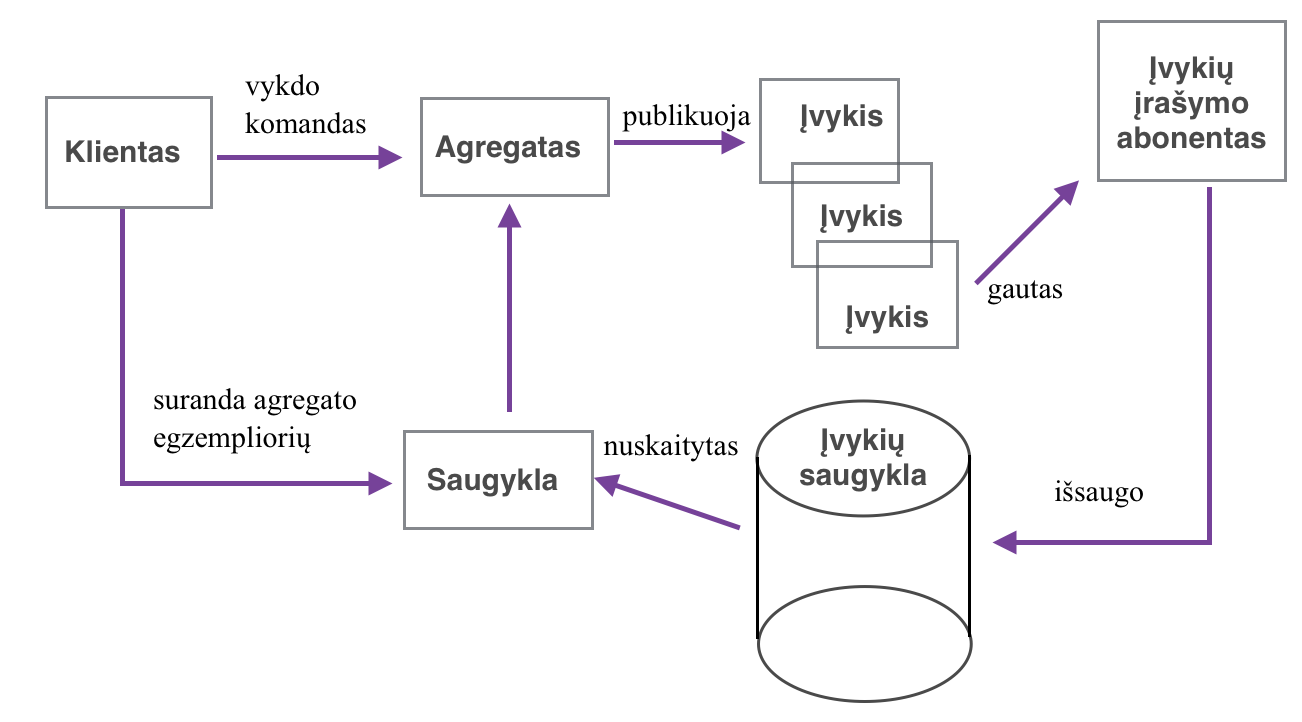
\includegraphics[width=0.9\linewidth]{pics/es.png}
	\caption{Įvykių kaupimo aukšo lygio reprezentacija}
	\label{pic:es}
\end{figure}

\subsubsection{Momentinė kopija}

Ilgame periode sistemoje susikaupia daugybė įvykių. Atkuriant agregato būseną reikia atkartoti šimtus, tūkstančius ar net milijonus įvykių. Tai tampa šio modelio silpnąja puse, nes įvykių atkartojimas užtrunka vis ilgiau sistemai plečiantis.

Tačiau šio duomenų kamsčio galima išvengti naudojant agregato būsenos momentines kopijas. Tam tikrame įvykių saugyklos istorijos taške yra padaroma agregato būsenos kopija. Serializuota agregato būsena yra įrašoma į įvykių saugyklą. Nuo to momento, agregatas yra atkuriamas pirmiausia naudojantis naujausia jo būsenos momentine kopija ir tik po to atkartojami visi naujesni įvykiai.

Momentinės kopijos nėra atkuriamos atsitiktinai. Jos gali būti kuriamos kas apibrėžtą skaičių įvykių. Šis skaičius turėtų būti parinktas analizuojant domeno sritį bei sistemą ir radus optimalų variantą. Tikėtinai gali būti 50 arba 100 įvykių tarp momentinių kopijų.

\subsubsection{Įvykių kaupimo privalumai ir trūkumai}

Kaip saugojimo mechanizmas, įvykių kaupimas stipriai skiriasi ir pakeičia ORM\footnote{http://www.orm.net/} įrankį. Kadangi įvykiai dažnai įrašomi kaip dvejetainės reprezentacijos, jie negali būti optimaliai naudojami užklausoms atlikti. Faktiškai įvykių kaupimu pagrįstoms saugykloms tereikia vienos operacijos - gauti įrašus pagal unikalią agregato tapatybę. To pasekoje užklausom daryti reikia kito kelio. Dažniausiai tam pasirenkamas CQRS\footnote{http://martinfowler.com/bliki/CQRS.html} principas. 

Įvykių kaupimas verčia kitaip mąstyti apie domeno modelį. Įvykių istorija gali padėti surasti bei ištaisyti sistemos defektus bei klaidas. Derinimas naudojant istoriją visų veiksmų, kurie nutiko sistemoje, turi didžiulį pranašumą. Įvykių kaupimas gali vesti prie didelio našumo domeno modelių, tai yra palaikyti ypač didelį skaičių operacijų per sekundę. Pavyzdžiui, įrašymas į vieną duomenų saugyklos lentelę yra ypač greitas. Negana to, tai leidžia CQRS užklausų modelį išplėsti horizontaliai, nes duomenų šaltinio atnaujinimai įvykdomi fone, kai įvykių saugykla yra atnaujinama naujais įvykiais.

\subsubsection{Įvykių kaupimas funkciniame programavime}

Vaughn Vernon pateikia keletą pastebėjimų apie įvykių kaupimą funkciniame programavime, kurie gali būti naudingi atliekant projektinius sprendimus bei eksperimentinį tyrimą:

\begin{itemize}

	\item Agregatas projektuojamas kaip nekintantis būsenos įrašas kartu su funkcijomis, kurios keičia būseną. Šios funkcijos paprasčiausiai priima būsenos įrašą ir įvykių argumentus ir gražina naują būsenos įrašą kaip rezultatą. Tokios funkcijos atrodo:

\begin{lstlisting}

	Funkcija<Busena, Ivykis, Busena>

\end{lstlisting}

	\item Dabartinė agregato būsena gali būti apibrėžta kaip suskleidimas į kairę visų praeities įvykių, kurie yra perduodami būseną keičiančiai funkcijai.

	\item Agregato metodai gali būti išreikšti kaip kolekcija funkcijų be būsenos.

	\item Įvykių saugykla gali būti suvokiama bei naudojama kaip funkcinė duomenų bazė, nes ji perduoda argumentus funkcijoms, kurios keičia agregato būseną. Momentinės kopijos įvykių saugykloje primena įsiminimą atmintyje\footnote{http://en.wikipedia.org/wiki/Memoization} funkciniame programavime.

\end{itemize}

\subsection{Monados}

\subsubsection{Terminas}

Funkciniame programavime monada yra struktūra, kuri atspindi skaičiavimus, apibrėžtus kaip seka žingsnių. Tipas kartu su monados struktūra apibrėžia ką reiškia vykdyti operacijas viena po kitos bei naudoti to pačio tipo įdėtines funkcijas. Tai leidžia kurti komandų grandines, kurios pažingsniui apdoroja informaciją, kur kiekvienas veiksmas yra dekoruojamas naujomis apdorojimo taisyklėmis, kurias apibrėžia monada \cite{OSullivan:2008:RWH:1523280}.

taisykles?

\subsection{Išvados}

Literatūros analizės metu remiantis kitų autorių patirtimi:

\begin{itemize}

\item išnagrinėtas funkcinis-reaktyvus programavimas,

\item išnagrinėtas įvykių kaupimo principas,

\item išnagrinėti įvykių srautai,

\item susipažinta su įvykių kaupimu funkciniame programavime,

\item susipažinta su monadomis,

\item įvaldyta sąvokų sistema, susijusi su nagrinėjama tematika.

\end{itemize}


\section{Sąvokų apibrėžimai}
\begin{itemize}

	\item \textbf{Agregatas} (angl. aggregate) - DDD modelis, rinkinys domeno objektų, kurie gali būti laikomi kaip visuma.

	\item \textbf{Derinimas} (angl. debugging) - riktų bei klaidų paieška programinėje įrangoje bei jų taisymas.

	\item \textbf{Esybė} (angl. entity) - kažkas, kas egzistuoja pats savaime, faktiškai arba hipotetiškai.

	\item \textbf{Horizontalus išplečiamumas} (angl. horizontal scaling) – galimybė sujungti daugybę techninės ar programinės įrangos esybių taip, jog jos dirbtų kaip visuma. Pavyzdžiui, galima pridėti keletą serverių pasinaudojant grupavimu arba apkrovos paskirstymu taip pagerinant sistemos našumą bei prieinamumą.

	\item \textbf{Metaduomenys} (angl. metadata) - duomenys apie kitus duomenis.

	\item \textbf{Tapatybės funkcija} (angl. identity function) - funkcija be jokio poveikio (ji visada grįžta ir jos argumentai tos pačios reikšmės).

	\item \textbf{Valentingumas} (angl. arity) - funkcijos valentingumas yra argumentų kiekis, kurį ji priima.

\end{itemize}

\section{Santrumpos ir paaiškinimai}
\begin{itemize}

	\item 1

	\item \textbf{CQRS} (angl. Command Query Responsibility Segregation) – komandų-užklausų atsakomybių atskyrimas.

	\item \textbf{DDD} (angl. Domain-Driven Design) – būdas kurti programinę įrangą, skirtą spręsti sudėtingus uždavinius, bei apjungti realizaciją kartu su augančiu domeno modeliu.

	\item \textbf{NoSQL} – duomenų bazė, skirta architektūriniams modeliams, kuriems nereikia palaikyti stiprios darnos principo, kuris naudojamas reliacinėse duomenų bazėse. Tai įgalina horizontalų išplečiamumą bei aukštesnį prieinamumą.

\end{itemize}

\bibliography{references}

\end{document}
